\documentclass[10pt, a4paper]{report}

\usepackage[utf8]{inputenc}
\usepackage[spanish]{babel}
\usepackage{amsfonts}
\usepackage{amsmath}
\usepackage{amssymb}
\usepackage{graphicx}
\usepackage{pdfpages}
\usepackage{spverbatim}
\usepackage[left=3.5cm,right=1.5cm,top=2.5cm,bottom=2.5cm]{geometry}
\usepackage{listings}
\usepackage{hyperref}
\author{Daniel Fernández Villanueva}
\title{Sistema de monitorización inercial del movimiento de las extremidades superiores}

\makeatletter
\renewcommand*{\UTFviii@defined}[1]{%
  \ifx#1\relax
    \begingroup
      % Remove prefix "\u8:"
      \def\x##1:{}%
      % Extract Unicode char from command name
      % (utf8.def does not support surrogates)
      \edef\x{\expandafter\x\string#1}%
      \StringEncodingConvert\x\x{utf8}{utf16be}% convert to UTF-16BE
      % Hexadecimal representation
      \EdefEscapeHex\x\x
      % Enhanced error message
      \PackageError{inputenc}{Unicode\space char\space \string#1\space
                              (U+\x)\MessageBreak
                              not\space set\space up\space
                              for\space use\space with\space LaTeX}\@eha
    \endgroup
  \else\expandafter
    #1%
  \fi
}
\makeatother

\setcounter{tocdepth}{3}
\usepackage{color}
\definecolor{dkgreen}{rgb}{0,0.6,0}
\definecolor{gray}{rgb}{0.5,0.5,0.5}
\definecolor{mauve}{rgb}{0.58,0,0.82}
\lstset{frame=tb,
  language=C++,
  aboveskip=3mm,
  belowskip=3mm,
  showstringspaces=false,
  columns=flexible,
  basicstyle={\small\ttfamily},
  numbers=left,
  frame=single,
  numberstyle=\tiny\color{gray},
  keywordstyle=\color{blue},
  commentstyle=\color{dkgreen},
  stringstyle=\color{mauve},
  breaklines=true,
  breakatwhitespace=true
  tabsize=4
}

\begin{document}

\maketitle

\tableofcontents

%%% ================ PARTE 1 : MEMORIA ================ %%%

\part{Memoria}

\pagestyle{headings}


%% ******** Capítulo 1 ******** %%

\chapter{ANTECEDENTES}


%% ******** Capítulo 2 ******** %%

\chapter{OBJETIVO DEL PROYECTO}

Este proyecto tiene como objetivo la implementación de un sistema de monitorización en tiempo real del movimiento de las extremidades superiores del cuerpo humano. Para la realización de este sistema se tendrá que dar solución a los siguientes

\begin{enumerate}
\item \textbf{Aplicación para la adquisición de datos de los sensores inerciales}: \\
Realización de un sistema que permitirá obtener en tiempo real los datos que proporcionan los sensores. En concreto se desarrollará un driver para un sensor xsens o una red de sensores xsens conectados mediante un master xbus. Este driver permitirá leer los datos que proporcionan los acelerómetros, giróscopos, magnetómetros y sensores de temperatura, además de la orientación de cada uno de los sensores conectados al PC. Este driver se encargará también de crear una interfaz para la posterior utilización de los datos en otros programas de foma sencilla. \\

\item \textbf{Tratamiento de los datos para obtener los ángulos de rotación entre cada sensor}:\\
Una vez sea posible la adquisición de los datos con el driver anterior, se creará otro programa con el que se obtendrán los ángulos de rotación entre cada sensor teniendo en cuenta además la geometría de las articulaciones del brazo o modelo sobre las que se situarán los sensores.\\

\item \textbf{Utilización de los datos para el objetivo deseado}: \\
En esta última fase se crearán los sistemas necesarios para la utilización de los datos con el objetivo deseado:

\begin{itemize}

\item Para la visualización de la posición del brazo en el simulador 3D Gazebo, se creará un modelo del brazo y una interfaz etre ROS y el simulador que permitirá la visualización de la posición del brazo en tiempo real.  

\item Para el control del robot mediante el movimiento del brazo o modelo del robot físico, se creará otra interfaz entre ROS y el driver del propio robot. 

\end{itemize}

\end{enumerate}


%%% ******** Capítulo 3 ******** %%%
\chapter{ESPECIFICACIONES DE DISEÑO}



%%% ******** Capítulo 4 ******** %%%
\chapter{DISEÑO DEL SISTEMA}

\section{Estudio de soluciones}
\section{Simulación}

%%% ******** Capítulo 3 ******** %%%
\chapter{IMPLEMENTACIÓN FÍSICA}
\section{Selección de componentes}
\section{Montaje}
\section{Ajuste}

\chapter{PROTOCOLO DE PRUEBAS. REDISEÑO}

\chapter{RESULTADOS OBTENIDOS}
%%% ******** Capítulo 5 ******** %%%
\chapter{HERRAMIENTAS UTILIZADAS}

En este capítulo se realizará una breve descripción de los elementos utilizados en el proyecto, tanto de hardware como de software.

\section{Hardware}

\subsection{Sensores XSENS}

\subsubsection{Sensor MTi-G}

\subsubsection{XBUS Master}

\subsection{Brazo humano}

\subsection{Robot Youbot}

\subsection{Modelo del robot Youbot}

\section{Software}

\subsection{ROS}

\subsubsection{¿Qué es ROS?}

ROS (del inglés \textit{Robot Operating System} - Sistema Operativo Robótico) es una plataforma de desarrollo de software que incluye conjunto de utilidades centradas en ayudar al desarrollador en la creación de programas para el control de robots. Esta herramienta incorpora abstracción del hardware, drivers para dispositivos, librerías, visualizadores, utilidades para el intercambio de mensajes entre programas y administradores de paquetes de software, entre otras muchas cosas. ROS es además software abierto, bajo una licencia BSD, por lo que cualquier persona puede ver su código fuente y modificarlo.

\subsubsection{¿Por qué usar ROS?}

ROS proporciona solución a diversos problemas que vienen dados inherentemente al objetivo de este proyecto:

\begin{itemize}

\item \textbf{Creación y compilación de programas}

\begin{itemize}

\item \textbf{Gestor de paquetes}

\end{itemize}

\item \textbf{Comunicación entre programas:}
ROS incluye:

\begin{itemize}

\item \textbf{Máster}

\item \textbf{Topics}

\item \textbf{Servicios}

\item \textbf{Servidor de parámetros}

\end{itemize}

\item \textbf{Visualización de datos}

\item \textbf{Otras herramientas}

\begin{itemize}

\item \textbf{Bag}

\item \textbf{rxplot}

\end{itemize}


\end{itemize}

\subsection{El sistema operativo Ubuntu}

\subsubsection{¿Qué es Ubuntu?}

Ubuntu es un sistema operativo con núcleo Linux. Es gratuito y es distribuido como software \textit{open source}. Se trata de la distribución GNU/Linux más popular en equipos personales

\subsubsection{¿Por qué usar Ubuntu?}

\subsection{El lenguaje de programación C++}



\subsection{Simulador Gazebo}

Gazebo es programa para simulación en 3D de un robot o una población de robots interactuando entre sí y el ambiente. Incorpora simulación de la física de sólidos rígidos y de la respuesta de sensores. Además incorpora un visualizador 3D bastante potente que permite ver en tiempo real la posición de los robots de forma realista.\\

La versión de Gazebo que se va a utilizar proporciona también una serie de herramientas para la comunicación con ROS. 
 

\subsection{Visualizador RViz}

\subsection{Control de versiones: git}

%%% ******** Capítulo 4 ******** %%%

\chapter{PROCESO DE REALIZACIÓN}

En este capítulo se detallará el proceso de realización de cada una de las fases del proyecto.

\section{Creación del driver para la adquisición de datos de los sensores xsens}

En está primera fase se tratará de encontrar un método para la toma de datos de la red de sensores inerciales. Estos sensores estarán conectados a un máster, que irá conectado al PC mediante conexión USB. Los datos así obtenidos se publicarán en \textit{topics} de ROS.

\subsubsection{Método seguido}

Para la realización del driver se ha partido del código incluido en la documentación de los sensores

\subsection{El paquete xsens\_driver}



\section{Creación de una librería matemática en C++ que permita trabajar con posiciones y orientaciones}


\subsection{La librería dfv}

\subsubsection{La clase Quaternion}

\subsubsection{La clase Vector3}

\subsubsection{La clase Matrix}

\section{Cálculo de los ángulos formados entre cada sensor}

\subsection{Formas de representar orientaciones espaciales}

Se puede configurar el sensor xsens para que proporcione una de las siguientes representaciones de su orientación:

\begin{itemize}

\item Ángulos de Euler.
\item Matriz de rotación.
\item Cuaternión. 

\end{itemize}

\subsubsection{Ángulos de Euler}
\subsubsection{Matrices de rotación}
\subsubsection{Cuaterniones}

\subsection{Utilización de cuaterniones para la representación de rotaciones}

Sea un vector unitario:

$$ \vec{e} = e_x i + e_y j + e_z k, \quad \|e\| = \sqrt{e_x^2 + e_y^2 + e_z^2} = 1 $$

Se definirá el cuaternión de rotación con ángulo $\theta$ sobre el eje dado por el vector $\vec{e}$:

$$ q(\theta, \vec{e}) = \cos \left(\frac{\theta}{2}\right) + \sin \left(\frac{\theta}{2}\right) e_x i + \sin \left(\frac{\theta}{2}\right) e_y j + \sin \left(\frac{\theta}{2}\right) e_z k$$

Se puede descomponer el cuaternión como suma de un número real y un cuaternión imaginario puro multiplicado por otro número real:

$$ q(\theta, \vec{e}) = \cos \left(\frac{\theta}{2}\right) + \sin \left(\frac{\theta}{2}\right) e  $$

Donde $e$ es el cuaternión imaginario puro (parte real nula) cuyas componentes se corresponden a las del vector unitario $\vec{e}$ que define el eje de rotación.\\

Por cuestión de comodidad:

$$ c_i = \cos \left( \frac{\theta_i}{2} \right) $$

$$ s_i = \sin \left( \frac{\theta_i}{2} \right) $$

De tal forma que ahora el cuaternión se escribirá de la siguiente manera:

$$ q(\theta_i, \vec{e_i}) = c_i + s_i e_i $$

El producto de dos cuaterniones se puede expresar de esta forma:

$$ q_1 q_2 = \left( c_1 + s_1 e_1 \right) \left( c_2 + s_2 e_2 \right) = c_1 c_2 + c_1 s_2 e_2 + c_2 s_1 e_1 + s_1 s_2 e_1 e_2 $$

El conjugado del cuaternión se representará de la siguiente manera:

$$ conj(q) = q^* $$

Dado a que se va a trabajar siempre con cuaterniones unitarios (también llamados \textit{versores}), se podrá asumir lo siguiente:

$$ \|q\| = 1 , \quad q^{-1} = \frac{q^*}{\|q\|^2} = q^* $$

De tal forma que:

$$ qq^* = q^*q = 1 $$

\subsubsection{Rotación de un vector alrededor de un eje y un ángulo dados}

Se puede realizar la rotación de un vector alrededor de un eje $\vec{e}$ y un ángulo $\theta$ mediante la siguiente operación:

$$ p' = q_1pq_1^*, \quad q_1 = q(\theta_1, \vec{e_1})$$

Si multiplicamos a la izquierda por $q_1^*$ y por la derecha por $q_1$:

$$ q_1^*p'q_1 = q_1^*(q_1pq_1)q_1^* $$ 

$$ q_1^*p'q_1 = p $$

Obtenemos que el conjugado representa una rotación inversa a la del cuaternión original:

$$ q^* = q\left(\theta, -\vec{e} \right) = q\left(-\theta, \vec{e}\right)  $$

\subsubsection{Composición de rotaciones en coordenadas extrínsecas}

El cuaternión de rotación definido por $q\left(\theta, \vec{e}\right)$ representa una rotación alrededor de un eje $\vec{e}$ fijo al sistema de referencia global.\\

Realizando una nueva rotación al vector obtenido anteriormente, se obtendrá una rotación compuesta por una primera rotación definida por el cuaternión $q_1$ seguida de otra rotación definida por $q_2$:

$$ p'' = q_2p'q_2^*, \quad q_2 = q(\theta_2, \vec{e_2})$$

$$ p'' = q_2(q_1pq_1^*)q_2^* = (q_2q_1)p(q_1^*q_2^*) = q_{12}pq_{12}^* $$

Se puede expresar la composición de dos rotaciones como un nuevo cuaternión que resulta de la multiplicación en orden inverso de los cuaterniones que definen las dos rotaciones:

$$ q_{12} = q_2q_1 $$

De aquí se obtiene que el conjugado del producto de dos cuaterniones es el producto de los conjugados en orden inverso:

$$ q_{12} = \left(q_2q_1\right)^* = q_1^*q_2^* $$

De forma análoga, para $n$ cuaterniones:

$$ q_{12 \dotsc (n-1)n} = q_nq_{n-1} \dotsm q_2q_1 $$
$$ q_{12 \dotsc (n-1)n} = \left( q_nq_{n-1} \dotsm q_2q_1 \right)^* = q_1^*q_2^* \dotsm q_{n-1}^*q_n^* $$

\subsubsection{Composición de rotaciones en coordenadas intrínsecas}



\subsubsection{Relación entre rotaciones intrínsecas y extrínsecas}

A continuación se demostrará que una rotación compuesta por varias rotaciones en el sistema de coordenadas intrínseco del sólido rígido se corresponde a la composición de rotaciones en el sistema extrínseco realizadas en orden inverso.\\

Se define un cuaternión de rotación asociado al eje intrínseco $\vec{e_2}$ después de haber sufrido una rotación definida por el cuaternión $q_1 = q\left( \theta_1 , \vec{e_1} \right)$ como:

$$ q_{2}^I = q\left(\theta_2 , \vec{e_2}^I \right) , \quad \vec{e_2}^I = (q_1e_2q_1^*)_{\vec{v}} $$ 

La orientación de partida es la misma para el sistema intrínseco y el extrínseco, por lo tanto:

$$ q_1^E = q_1^I = q_1 $$

Para demostrar la afirmación de partida se tendrá que demostrar la veracidad de la siguiente igualdad:

$$ q_2^Iq_1 = q_1q_2^E $$

Se reordenará la igualdad para que los cálculos sean más sencillos:

$$ q_2^Iq_1 = q_1q_2^E \iff q_2^I = q_1q_2^Eq_1^* $$

Desarrollo del lado izquierdo de la igualdad:

$$ q_2^I = c_2 + s_2(q_1e_2q_1^*) $$

$$ q_1e_2q_1^* = (c_1 + s_1e_1)e_2(c_1 - s_1e_1) = (c_1e_2 + s_1e_1e_2)(c_1 - s_1e_1) = $$

$$ = c_1^2e_2 + s_1c_1e_1e_2 - c_1s_1e_2e_1 - s_1^2e_1e_2e_1 = c_1^2e_2 + s_1c_1(e_1e_2 - e_2e_1) - s_1^2e_1e_2e_1 $$

\section{Incorporación de las herramientas creadas}

\subsection{Visualizador de la posición del brazo}

\subsubsection{Obtención de los ángulos de rotación entre cada segmento del brazo}

\subsubsection{Cálculo de las posiciones de cada segmento del brazo}

\subsubsection{Implementación}

\subsection{Controlador de un simulador del brazo robótico del robot Youbot}

\subsection{Controlador del brazo robótico del robot Youbot real}

%%% ******** Capítulo 5 ******** %%%

\chapter{RESULTADOS EXPERIMENTALES}


%%% ******** Capítulo 6 ******** %%%

\chapter{CONCLUSIONES}


%%% ******** Capítulo 7 ******** %%%

\chapter{BIBLIOGRAFÍA}


%%% ================ PARTE 2 : ANEXOS ================ %%%

\part{Anexos}

\appendix

\chapter{INSTALACIÓN Y PUESTA EN MARCHA DEL SOFTWARE}

\chapter{SOLUCIÓN DE PROBLEMAS}

\section{Error iniciando Gazebo}

\begin{spverbatim}
Msg Waiting for master
Msg Connected to gazebo master @ http://localhost:11345
Exception [Master.cc:69] Unable to start server[Address already in use]


terminate called after throwing an instance of 'gazebo::common::Exception'
Aborted (core dumped)
[gazebo-1] process has died [pid 2795, exit code 134, cmd /opt/ros/fuerte/stacks/simulator_gazebo/gazebo/scripts/gazebo /opt/ros/fuerte/stacks/simulator_gazebo/gazebo_worlds/worlds/empty.world __name:=gazebo __log:=/home/daniel/.ros/log/772c2f96-ab75-11e2-a2fc-001de05009b5/gazebo-1.log].
log file: /home/daniel/.ros/log/772c2f96-ab75-11e2-a2fc-001de05009b5/gazebo-1*.log
LightListWidget::OnLightMsg
\end{spverbatim}

\textbf{Solución: }
Ejecutar comando:
\begin{verbatim}
$ ps ax | grep [g]z
\end{verbatim}

Ver si hay un proceso gzserver

\begin{spverbatim}
 3118 ?        Sl    12:47
 /opt/ros/fuerte/stacks/simulator_gazebo/gazebo/gazebo/bin/gzserver 
 /opt/ros/fuerte/stacks/simulator_gazebo/gazebo_worlds/worlds/empty.world __name:=gazebo __log:=/home/daniel/.ros/log/8188cc76-ab73-11e2-a4ec-001de05009b5/gazebo-1.log -s /opt/ros/fuerte/stacks/simulator_gazebo/gazebo/lib/libgazebo_ros_paths_plugin.so -s /opt/ros/fuerte/stacks/simulator_gazebo/gazebo/lib/libgazebo_ros_api_plugin.so
\end{spverbatim}

Si lo hay, ejecutar \textit{System Monitor} y matar el proceso \textit{gzserver}.

\chapter{Instalación y configuración del software necesario}

\section{Instalación de ROS Fuerte}

La versión de ROS que se utilizará es ROS Fuerte. Esta elección se debe a que dicha versión es compatible con el simulador Gazebo, con el que posteriormente se realizará la visualización en 3D del modelo.\\

Para realizar la instalación de ROS  se partirá de una instalación previa de Ubuntu, pudiendo ser éste de cualquiera de estas \textit{releases}:

\begin{itemize}
\item 10.04 LTS (Lucid Lynx)
\item 11.04 (Oneiric Ocelot)
\item 12.04 LTS (Precise Pangolin)
\end{itemize}

\subsection{Configuración de los repositorios de Ubuntu}

Se procederá a abrir el Centro de Sofware de Ubuntu y en la barra de menú de dicho programa, se seleccionará en el menú Edit la opción Software Sources. En la pestaña Ubuntu Software se comprobará que están seleccionados los repositorios restricted, universe y multiverse:\\

%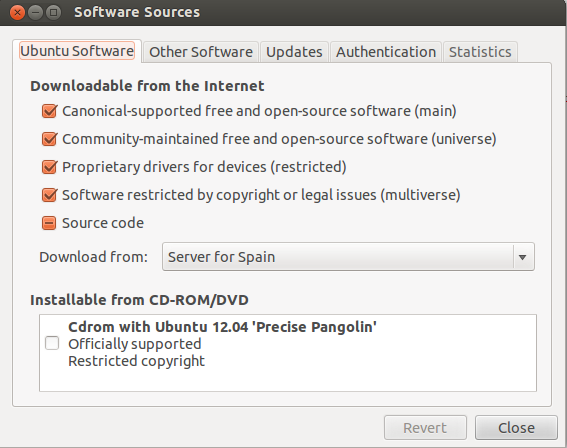
\includegraphics[scale=0.5]{../img/Software sources.png} 

\subsection{Configuración del archivo sources.list}

El archivo sorces.list le dice al gestor de paquetes de Ubuntu de dónde puede obtener cada paquete de ROS.
Se abrirá un terminal y se ejecutará el siguiente comando que dependerá de la versión de Ubuntu que tengamos instalada:\\

\textbf{Ubuntu 10.04 (Lucid)}
\begin{verbatim}
$ sudo sh -c 'echo "deb http://packages.ros.org/ros/ubuntu lucid main" 
> /etc/apt/sources.list.d/ros-latest.list'
\end{verbatim}

\textbf{Ubuntu 11.10 (Oneiric)}
\begin{verbatim}
$ sudo sh -c 'echo "deb http://packages.ros.org/ros/ubuntu oneiric main" 
> /etc/apt/sources.list.d/ros-latest.list'
\end{verbatim}

\textbf{Ubuntu 12.04 (Precise)}
\begin{verbatim}
$ sudo sh -c 'echo "deb http://packages.ros.org/ros/ubuntu precise main" 
> /etc/apt/sources.list.d/ros-latest.list'
\end{verbatim}

Este comando lo que hace es crear un archivo de texto en la ruta especificada como parámetro, que contiene la dirección de donde descargar los paquetes para la versión específica de ROS que tengamos.

\subsection{Configuración de la keys}

En el terminal se ejecutará el siguiente comando:

\begin{verbatim}
$ wget http://packages.ros.org/ros.key -O - | sudo apt-key add -
\end{verbatim}

\subsection{Descarga e instalación}

Se actualizará el índice de paquetes de Ubuntu para tener la seguridad de que el servidor de ROS.org está indexado:

\begin{verbatim}
$ sudo apt-get update
\end{verbatim}

A continuación se procederá a descargar e instalar la versión completa de ROS. El el terminal se ejecutará el siguiente comando:

\begin{verbatim}
$ sudo apt-get install ros-fuerte-desktop-full
\end{verbatim}

Esta instalación traerá consigo las siguientes herramientas, entre otras:

\begin{itemize}
\item ROS
\item rx (herramientas para interfaz gráfica: rxbag,  rxgraph, rxplot, ...)
\item rviz (herramienta de visualización 3D)
\item librerías genéricas para robots
\item Simuladores 2D/3D (entre ellos Gazebo)
\item Navegación y percepción 2D y 3D
\end{itemize}

\subsection{Configuración del entorno}

Cada vez que se inicie un nuevo terminal es necesario añadir las variables de entorno. Si se quisiera, se puede automatizar dicha tarea ejecutando el comando:

\begin{verbatim}
$ echo “source /opt/ros/fuerte/setup.bash” >> ~/.bashrc
\end{verbatim}

Este comando añade la línea  source /opt/ros/fuerte/setup.bash al archivo ~/.bashrc. Este archivo contiene la configuración inicial del terminal, y se ejecuta cada vez que abrimos un nuevo terminal. Posteriormente se ejecutará el archivo anterior para actualizar el terminal. De esta forma reconocerá los nuevos comandos de ROS:

\begin{verbatim}
$ . ~/.bashrc
\end{verbatim}

\subsection{Otras herramientas}

Se instalarán dos herramientas que permitirán obtener los paquetes necesarios para obtener los datos de los sensores XSENS MTi-G. Para ello, en el terminal se ejecutará el siguiente comando:

\begin{verbatim}
$ sudo apt-get install python-rosinstall python-rosdep
\end{verbatim}

\section{Instalación del simulador Gazebo}

Para instalar la versión de Gazebo preparada para comunicarse con ROS se ejecutará el siguiente comando:

\begin{verbatim}
$ sudo apt-get install ros-fuerte-simulator-gazebo
\end{verbatim}


\chapter{CÓDIGO FUENTE}

\section{Driver Xsens}

\subsection{xsens\_node.cpp}
%\lstinputlisting[language=C++]{../../xsens_driver/src/xsens_node.cpp}
\newpage

\part{Otros documentos}

\section{Manual del sensor MTi-G}

%\includepdf[pages={-}]{doc/mtig_manual.pdf}
AAAAAAAAAAAAAAAAAAAAAAa

\end{document}
